\documentclass{article}
\usepackage[utf8]{inputenc} % Para caracteres en español
\usepackage{amssymb}
\usepackage{amsmath}
\usepackage{indentfirst}
\usepackage{graphicx}
\usepackage{caption}
\usepackage{float}
\graphicspath{{image_test/}{out_test/}}
%\usepackage[brazil]{babel}
\setlength{\parindent}{1cm}
\newcommand\tab[1][1cm]{\hspace*{#1}}
\renewcommand*\contentsname{Índice}
 
% capa
\begin{document}
	\begin{titlepage} %iniciando a "capa"
	\begin{center} %centralizar o texto abaixo
	{\large Universidade de São Paulo}\\[0.2cm] %0,2cm é a distância entre o texto dessa linha e o texto da prox
	{\large Instituto de Matemática e Estatística}\\[0.2cm] % o comando \\ "manda" o texto ir para próxima linha
	{\large MAC0210}\\[5.1cm]
	{\bf \huge Relat\'orio: Exerc\'icio-Programa 2}\\[5.1cm] % o comando \bf deixa o texto entre chaves em negrito. O comando \huge deixa o texto enorme
	\end{center} %término do comando centralizar
	{\large Alunos:}\\ 
	{Gustavo Silva \tab\tab\tab No USP: 9298260\\
	 Leonardo Padilha \tab\tab\tab No USP: 9298295}\\[0.7cm] % o comando \large deixa o texto grande
	{\large Professor: Ernesto G. Birgin}\\[5.1cm]
	\end{titlepage} %término da "capa"
	
	\tableofcontents
	\pagebreak
	\section{Objetivo}
	\setlength{\parindent}{10ex}
	Nosso objetivo nesse Exercício-Programa é gerar um programa que comprima e descomprima uma dada imagem. \par
	Para comprimir, basta remover alguns pixels da imagem, mais precisamente, dado um número real $k$, e considerando que a imagem é uma matriz de pixels, então removemos as linhas e as colunas $i$ tais que $i \equiv 1\ \textrm{mod}(k + 1)$. \par
	Para fazer a descompressão, assumimos que a imagem é, basicamente, uma função que vai do $\mathbb{R}^2$ para o $\mathbb{R}^3$ ($\mathbb{R}^3$ pois estamos considerando a paleta RGB, logo, uma coordenada para cada cor da paleta) e, dessa forma, cada pixel vira um ponto no plano $\mathbb{R}^2$ (devemos considerar também que o espaçamento entre dois pixels adjacentes $h$ foi definido por nós). Agora, para inserirmos os novos pixels de coordenadas $(x, y) \in \mathbb{R}^2$ basta interpolarmos a função nessa região. \par
	Para fazer a interpolação, usamos dois métodos diferentes que são extensões para $\mathbb{R}^2$ dos métodos vistos em sala de aula. Vamos explicar e avaliar os resultados obtidos com cada um deles.
	
	\section{Interpolação Bilinear por partes}
	Esse método é uma extensão para $\mathbb{R}^2$ da interpolação linear de uma função de $\mathbb{R}$ para $\mathbb{R}$. \par
	Vamos considerar 4 pixels conhecidos adjacentes: $Q_{0}$, $Q_{1}$, $Q_{2}$ e $Q_{3}$. Esses pixels podem ser representados como pontos do plano $\mathbb{R}^2$ de coordenadas $(x_{i}, y_{j}), (x_{i+1}, y_{j}), (x_{i}, y_{j+1}), (x_{i+1}, y_{j+1})$, respectivamente onde $x_{i}, x_{i+1}, y_{j}, y_{j+1} \in \mathbb{R}$. Supondo que a imagem é uma amostra de uma função $f$ tal que $f: \mathbb{R}^2 \rightarrow \mathbb{R} $, então, para gerar um pixel que está em uma coordenada $(x_{0}, y_{0})$ tal que $x_{0} \in [x_{i}, x_{i+1}]$ e $y_{0} \in [y_{j}, y_{j+1}]$, podemos criar uma função interpoladora $v$, que interpola os valores no intervalo, dada por:
	 \begin{equation}
	 v(x, y) = c_{0} + c_{1}(x - x_{i}) + c_{2}(y - y_{j}) + c_{3}(x - x_{i})(y - y_{j})
	 \end{equation}
	 Que é a mesma coisa que:
	 \[
	 	\left[
	 		\begin{array}{llll}
				f(x_{i}, y_{j})\\
				f(x_{i+1}, y_{j})\\
				f(x_{i}, y_{j+1})\\
				f(x_{i+1}, y_{j+1})	 		
	 		\end{array}
	 	\right]
	 	=
	 	\left[
	 		\begin{array}{llll}
				1 & 0 & 0 & 0\\
				1 & h & 0 & 0\\
				1 & 0 & h & 0\\
				1 & h & h & h^2	 		
	 		\end{array}
	 	\right]
	 	\left[
	 		\begin{array}{llll}
				a_{0}\\
				a_{1}\\
				a_{2}\\
				a_{3}	 		
	 		\end{array}
	 	\right]
	 \]
	 Podemos, então, utilizar as funções do Octave para calcular os coeficientes rapidamente. \par
	 Na nossa implementação, selecionamos cada pixel conhecido e, para cada um da linha $i$ coluna $j$, definimos que ele é a origem do sistema de coordenadas, assim conseguimos simplificar as contas, já que os pixels adjacentes são $(0, h)$, $(h,0)$ e $(h,h)$ e teremos sempre as mesmas coordenadas dos pixels que queremos interpolar que serão os pontos tal que $(\dfrac{m}{k+1}h, \dfrac{n}{k+1}h)$ onde $m$, $n \in {1, 2, ..., k}$. Após isso, calculamos os coeficientes do polinômio $v$ e conseguimos interpolar todos os $(k+2)^2$ pontos que estão no quadrado definido entre o pixel conhecido da linha $i$ coluna $j$ e o pixel da linha $i+1$ coluna $j+1$, incluindo estes quatro pontos já conhecidos.\par
	 Para realizar esta interpolação, adaptamos a equação responsável por interpolar um ponto, que é dada por:
	 \[
	 	v(x,y) = 
	 	\left[
	 		\begin{array}{llll}
		 		1 & x & y & xy
	 		\end{array}
	 	\right]
	 	\left[
	 		\begin{array}{llll}
	 		c_{0}\\
	 		c_{1}\\
	 		c_{2}\\
	 		c_{3}
	 		\end{array}
	 	\right]
	 \]
	  para que ela pudesse, em uma única multiplicação matricial, nos retornar todos os pontos compreendidos entre $[0, h]$x$[0, h]$, em uma matriz quadrada $(k+2)$x$(k+2)$. \par
	  A equação que nos dá todos os pontos é:
	  \begin{equation}
	  \begin{aligned}
	  	\left[
	  	\begin{array}{cccc}
	  	
	  		v(x_{0}, y_{0}) & ... & v(x_{n}, y_{0})\\
	  		v(x_{0}, y_{1}) & ... & v(x_{n}, y_{1})\\
	  				       &  .  &    \\
	  				       &  .  &    \\
	  				       &  .  &    \\ 	
	  		v(x_{0}, y_{n}) & ... & v(x_{n}, y_{n})
	  			
	  	\end{array}
	  	\right]
	  	= 
	  	X
	  	\left[
	  		\begin{array}{cccc}
	  			c_{0}     & 0     & 0     & 0\\
	  			0         & c_{1} & 0     & 0\\
	  			0         &  0    & c_{2} & 0\\
	  			0         &  0    &   0   & c_{3} 
	  		\end{array}
	  	\right]
	  	Y
	  	\end{aligned}
	  \end{equation}\par 
	  Onde 
	  \[
	  	X = 
	  	\left[
  		\begin{array}{cccc}
  			1 & x_{0} & 1 & x_{0}\\
  			1 & x_{1} & 1 & x_{1}\\
				&.\\
				&.\\
				&.\\
  			1 & x_{n} & 1 & x_{n}\\
  		\end{array}
  	\right]
  	,Y =
	  	\left[
	  		\begin{array}{cccc}
	  			1     & 1     & ...     & 1\\
	  			1     & 1     & ...     & 1\\
	  			y_{0} & y_{1} & ...     & y_{n}\\
	  			y_{0} & y_{1} & ...     & y_{n}
	  		\end{array}
	  	\right]
	  \]
	  e $(x_{l}, y_{m})$ são as coordenadas dos novos pixels que queremos interpolar. Assim, para cada pixel conhecido na imagem (excetuando-se os da última linha e última coluna), calculamos os coeficientes da $v(x,y)$ que abrange o quadrado de lado $h$ formado por este pixel e seus vizinhos, e utilizamos esta multiplicação matricial para interpolar todos os pontos novos dentro do quadrado de uma só vez. Em seguida, esse quadrado é posicionado na matriz que receberá a imagem interpolada, no seu devido local. Ao final, a combinação de todos os quadrados terá gerado a imagem interpolada. \par
	 Com esse método, garantimos um custo de tempo quadrático ($\mathcal{O}(p^2)$ onde $p$ é a quantidade de pixels na vertical ou horizontal da imagem original) pois precisamos olhar para cada pixel da imagem.
		\subsection{Resultados no Zoológico}
		Nesses experimentos, executamos o método com 6 tipos diferentes de funções $\mathbb{R}^2 \rightarrow \mathbb{R}^3$ para a criação da imagem original, são elas:
		\[
			\begin{array}{llllll}
			1)\ f(x, y) = (\sin(\dfrac{1}{x-50}),\ \frac{e^x}{xy - 30},\ xy) \\
			2)\ f(x, y) = (\tan(xy - 10),\ \cos(x),\ \sin(\dfrac{1}{xy}) \\
			3)\ f(x, y) = (\dfrac{1}{\sqrt{xy - 10}},\ xy - 10,\ \cos(x^2 - 2xy + y^2)) \\
			4)\ f(x, y) = ((x - y)^2,\ x,\ y) \\
			5)\ f(x, y) = (\sin(x^2 - y^2), e^x + y^2, e^y - x^2) \\
			6)\ f(x, y) = (sen(x),\ \dfrac{sen(y) + sen(x)}{2}, sen(x)) \\
			\end{array}
		\]
		O intervalo que escolhemos para a criação da imagem relativa a essas funções foram de [0, 200]X[0, 200] com espaçamento de 0.5 entre os pontos. \par
		Perceba que as 3 primeiras funções não são de classe $C^1$ enquanto as 3 últimas são de classe $C^\infty$ no intervalo definido por nós. Isso é proposital, pois queremos verificar como a nossa interpolação funciona com funções de classe $C^2$. \par
		Nos nossos testes, percebemos que o erro não depende de $h$, por isso, vamos mostrar aqui apenas para $h = 1$. \par
		Vamos verificar o valor do erro da compressão e em seguida a descompressão com $k = 1$.
		\pagebreak
		\begin{figure}[H]
			\centering
			\captionsetup{justification=centering}
			
\includegraphics[width=100px]{/zoo/1.jpg} \ \ \
			
\includegraphics[width=100px]{/zoo/decompressed_1.png} \\
			\caption{À direita a imagem da função 1 original e à esquerda a imagem após passar pelo processo de compressão e descompressão com $k = 1$.}  
			
		\end{figure}\par
		O erro observado nessa primeira função foi de 5.5861\%. Podemos perceber que esse erro ocorre principalmente na parte esquerda da imagem, onde, na imagem original, existem algumas colunas onde a cor vai se suavizando para o azul e, na imagem após o processo, as colunas não possuem essa suavidade. Isso se dá pelo método adotado, que não interpola a função de forma "suave".
		
		\begin{figure}[H]
			\centering
			\captionsetup{justification=centering}
			
\includegraphics[width=100px]{/zoo/2.jpg} \ \ \
			
\includegraphics[width=100px]{/zoo/decompressed_2.png} \\
			\caption{Resultados com a função 2 (original à direita e à esquerda após o processo).}  
		\end{figure}\par
		Para a função 2, verificamos um erro de 1.8\% entre a imagem original e a imagem após o processo, o pequeno erro pode ser decorrente do fato de que a imagem gerada não possui muitas curvas, e assim a interpolação bilinear se torna suficiente.\par
		
		\begin{figure}[H]
			\centering
			\captionsetup{justification=centering}
			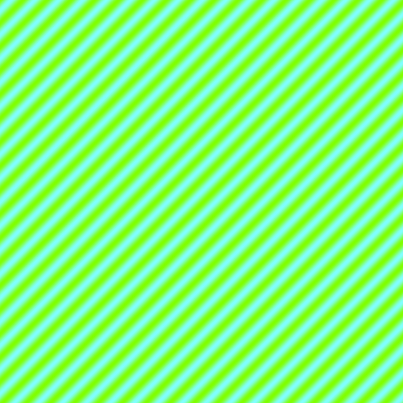
\includegraphics[width=100px]{/zoo/3.jpg} \ \ \
			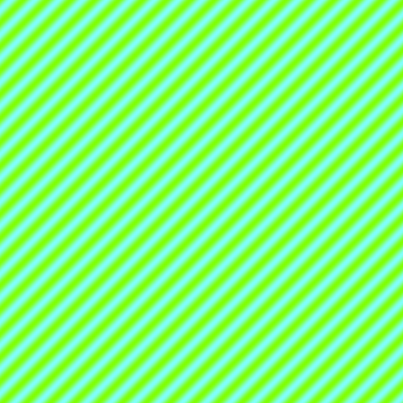
\includegraphics[width=100px]{/zoo/decompressed_3.png} \\
			\caption{À direita a imagem da função 3 original e à esquerda a imagem após passar pelo processo de compressão e descompressão com $k = 1$.}  
			\label{func3}
		\end{figure}\par
		Para a função 3, temos um erro de 0.74\%, provavelmente pelo mesmo motivo da função 2, ou seja, a imagem gerada pela função não possui curvas.
		
		\begin{figure}[H]
			\centering
			\captionsetup{justification=centering}
			
\includegraphics[width=100px]{/zoo/4.jpg} \ \ \
			
\includegraphics[width=100px]{/zoo/decompressed_4.png} \\
			\caption{À direita a imagem da função 4 original e à esquerda a imagem após passar pelo processo de compressão e descompressão com $k = 1$.}  
		\end{figure}\par
		A função 4 apresentou um erro de 0.8\%, um caso interessante, dado que a imagem apresenta algumas curvas. Porém, esse baixo erro deve ser causado pelo fato de que a imagem apresenta uma cor constante no centro, mudando apenas nas bordas de tal forma que a interpolação bilinear seja suficiente, o erro, porém, está nas bordas dos círculos dos cantos.
		
		\begin{figure}[H]
			\centering
			\captionsetup{justification=centering}
			
\includegraphics[width=100px]{/zoo/5.jpg} \ \ \
			
\includegraphics[width=100px]{/zoo/decompressed_5.png} \\
			\caption{À direita a imagem da função 5 original e à esquerda a imagem após passar pelo processo de compressão e descompressão com $k = 1$.}  
		\end{figure}\par
		O erro apresentado pela função 5 é de 1.24\%, provavelmente causado pela mudança de cor da parte superior da imagem.
		
		\begin{figure}[H]
			\centering
			\captionsetup{justification=centering}
			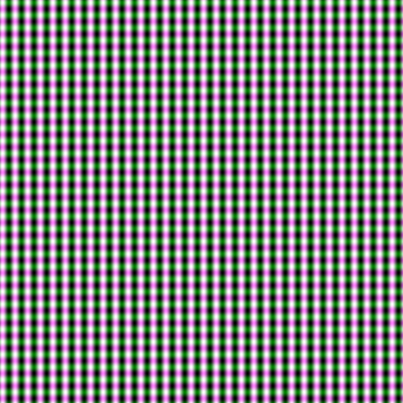
\includegraphics[width=100px]{/zoo/6.jpg} \ \ \
			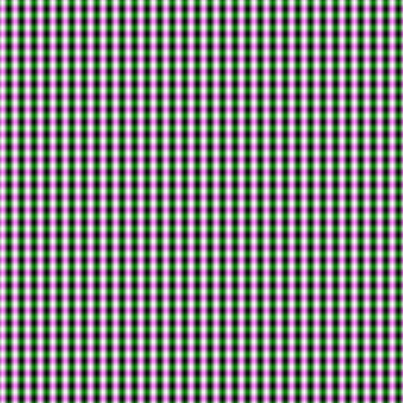
\includegraphics[width=100px]{/zoo/decompressed_6.png} \\
			\caption{À direita a imagem da função 6 original e à esquerda a imagem após passar pelo processo de compressão e descompressão com $k = 1$.}  
		\end{figure}\par
		A função 6, entretanto, apresentou um erro elevado (4.25\%), causado pelo fato da função ser muito suave (gerando várias mudanças de cores que ao interpolarmos usando o método bilinear, perderemos as informações).\par
		Percebemos, portanto, que a interpolação funciona bem com todo tipo de imagem (preto e branco ou colorido), com erro máximo de 5\% nos experimentos, mas apenas para $k = 1$, vamos ver abaixo um caso que torna o método ineficiente para um $k$ maior. É importante ressaltar que as funções de classe $C^2$ não apresentaram diferenças em relação àquelas que não são, pois a média dos erros das funções de classe $C^2$ foi semelhante à média dos erros das que não são de classe $C^2$.\par
		Por fim, fizemos mais alguns testes especificamente com a função 6: o primeiro foi comprimir e descomprimir com $k = 7$. Para isso, criamos uma imagem menor (para que exista a condição de existência de um $n$ natual tal que $p = n + (n-1)k$ onde $p$ é a quantidade de pixels) com 233x233 pixels e o intervalo da função passou a ser de $[0, 115]$x$[0, 115]$. O resultado segue abaixo:
		\begin{figure}[H]
			\centering
			\captionsetup{justification=centering}
			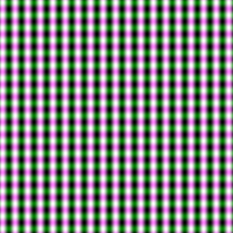
\includegraphics[width=100px]{/zoo/k7.jpg} \ \ \
			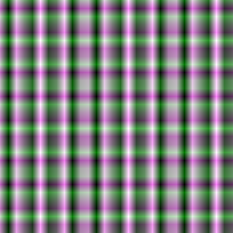
\includegraphics[width=100px]{/zoo/decompressed_k7.png} \\
			\caption{À direita a imagem da função 6 original e à esquerda a imagem após passar pelo processo de compressão e descompressão com $k = 7$.}  
		\end{figure}\par
		O erro com esse valor de $k$ subiu para 50\%! A causa está na compressão, que faz a imagem de 233x233 pixels para 30x30 pixels, perdendo muita informação e, ao recriarmos a imagem com o método bilinear, não obtemos as informações novamente, fazendo com que a diferença entre a imagem original e a imagem após o procedimento seja grande.\par
		Nosso último experimento foi rodar o compress três vezes com $k = 1$ (vale ressaltar que a imagem gerada aqui foi exatamente a mesma que a do último experimento, com $k = 7$) e em seguida decompress três vezes com $k = 1$. Obtemos os seguintes resultados: 
		\begin{figure}[H]
			\centering
			\captionsetup{justification=centering}
			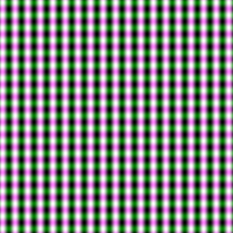
\includegraphics[width=100px]{/zoo/k7.jpg} \ \ \
			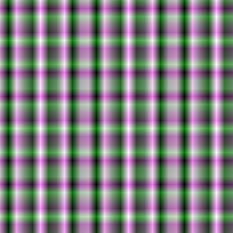
\includegraphics[width=100px]{/zoo/decompressed_k1-3.png} \\
			\caption{À direita a imagem da função 6 original e à esquerda a imagem após passar pelo processo de compressão e descompressão com $k = 1$ três vezes.}  
		\end{figure}\par
		O erro obtido dessa forma foi também de 50\% pelo mesmo motivo do último experimento: a imagem, ao ser comprimida, acaba perdendo muita informação (afinal, ao final dos três compress, obtivemos uma imagem de tamanho 30x30 pixels). \par
		Percebemos que o erro se comporta de acordo com $k$, ou seja, quanto mais comprimimos a imagem, maior o erro obtido. 
		
		\subsection{Resultados na Selva}
		Nesses experimentos, usamos 4 imagens: duas preto e branco e duas coloridas. O valor $k$ da compressão foi de 1. Abaixo temos os resultados obtidos:
		\begin{figure}[H]
			\centering
			\captionsetup{justification=centering}
			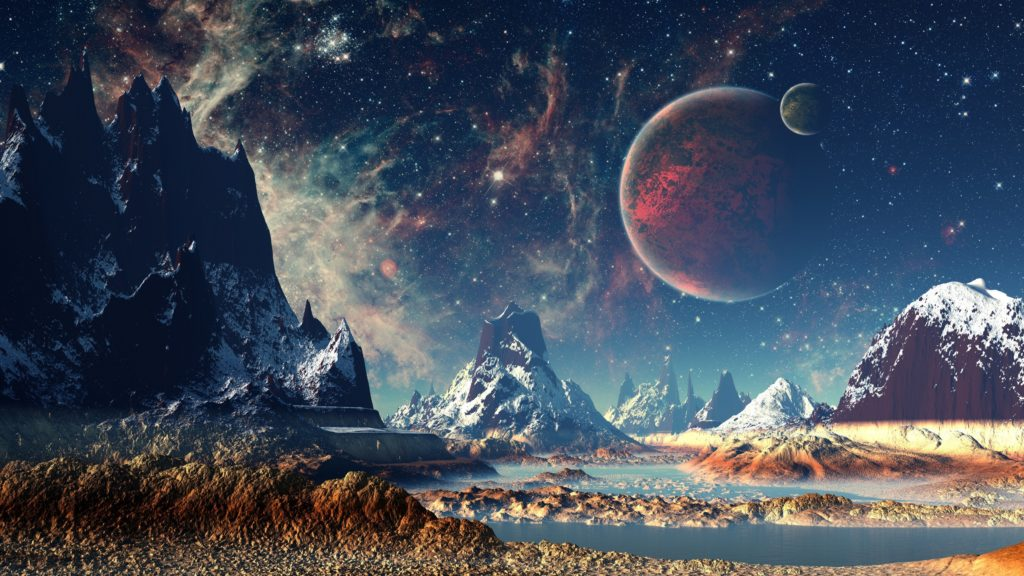
\includegraphics[width=100px]{/jungle/image01.jpg} \ \ \
			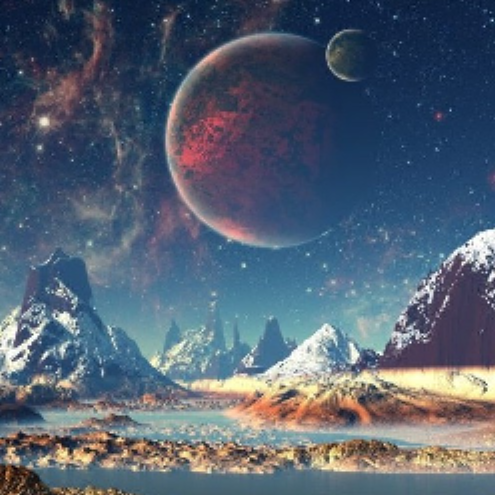
\includegraphics[width=100px]{/jungle/decompressed_11.png} \\
			\caption{À direita a imagem original e à esquerda a imagem após o processo. O erro obtido foi de 1.3\%.}  
		\end{figure}\par
		\begin{figure}[H]
			\centering
			\captionsetup{justification=centering}
			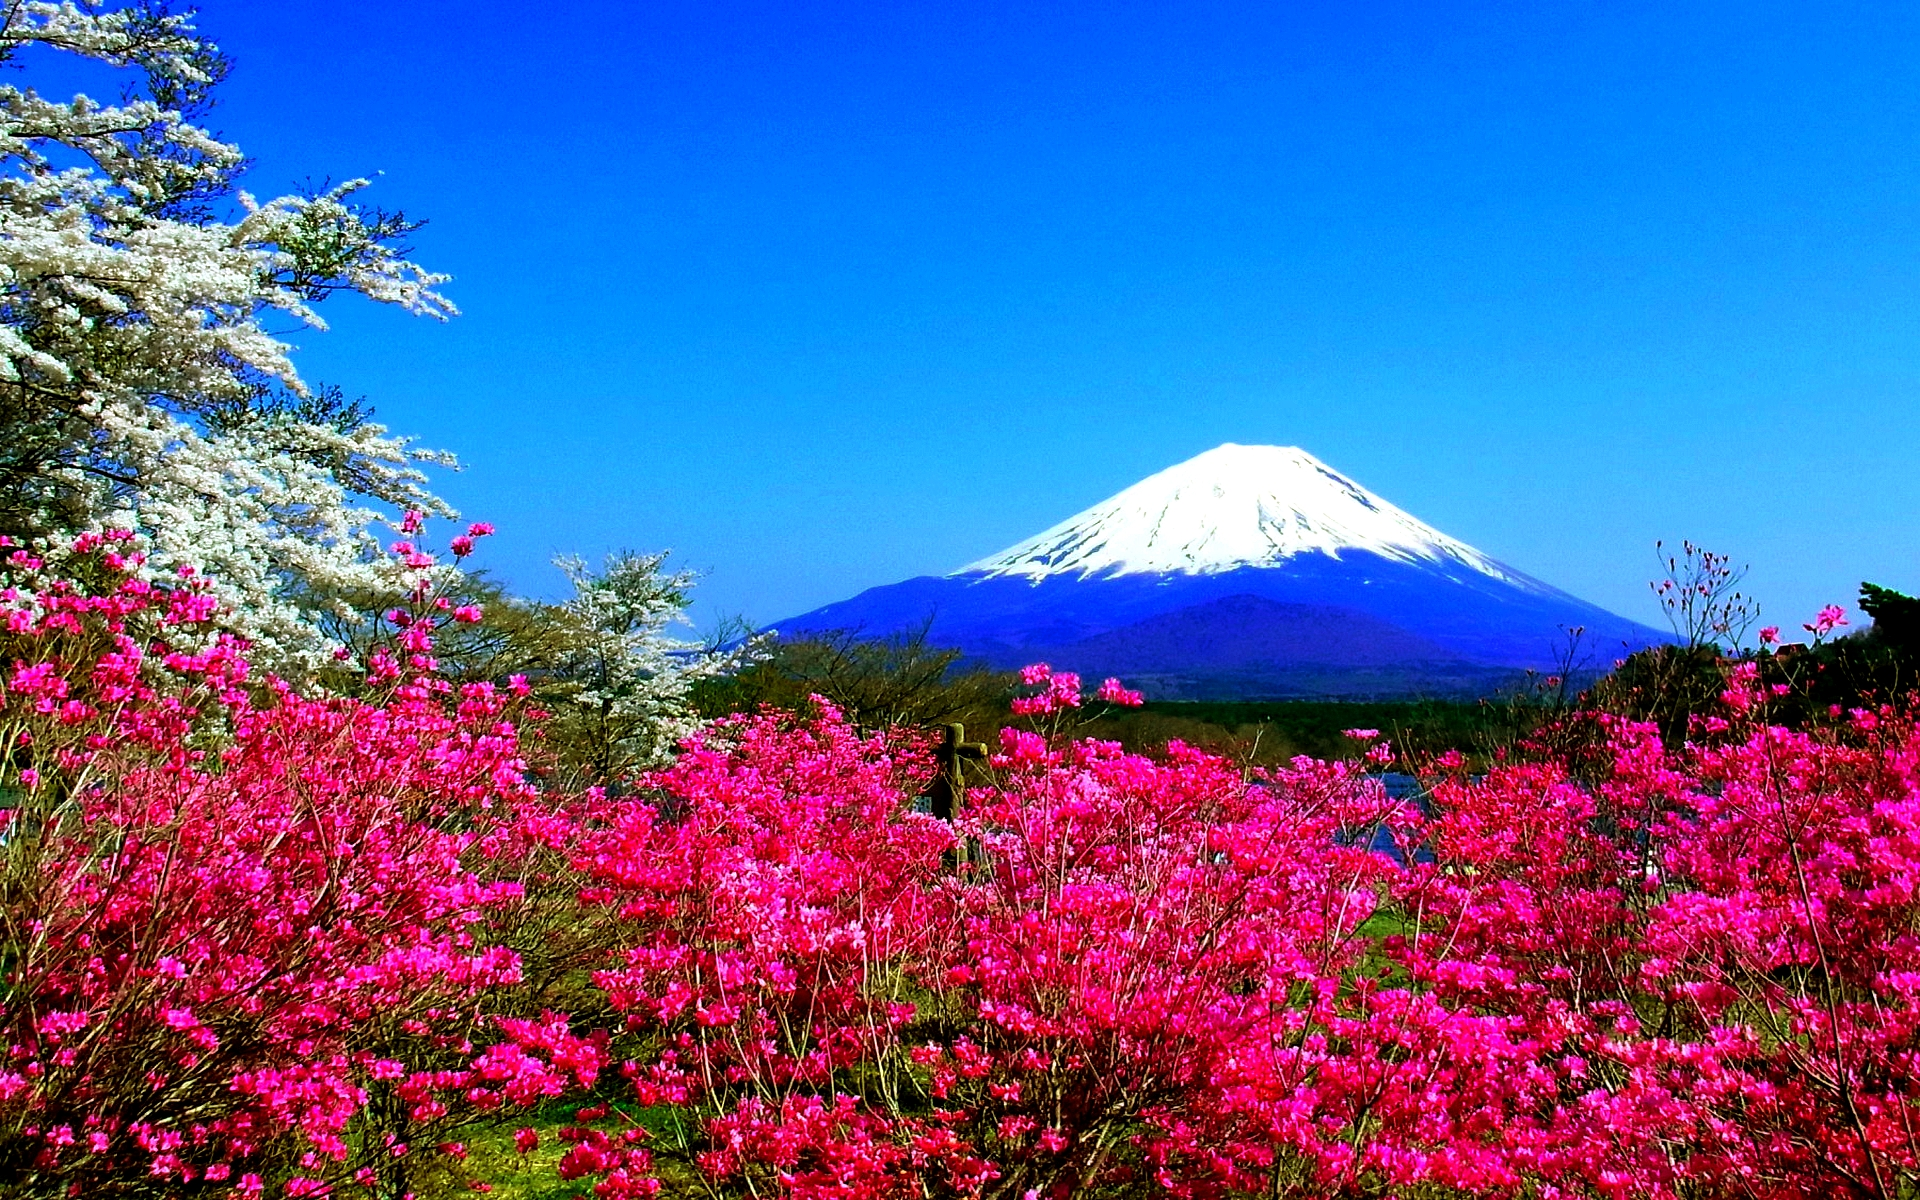
\includegraphics[width=100px]{/jungle/image02.jpg} \ \ \
			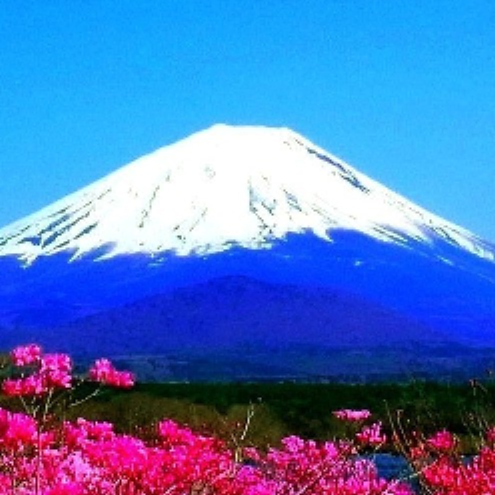
\includegraphics[width=100px]{/jungle/decompressed_12.png} \\
			\caption{À direita a imagem original e à esquerda a imagem após o processo. O erro obtido foi de 1\%.}  
		\end{figure}\par
		\begin{figure}[H]
			\centering
			\captionsetup{justification=centering}
			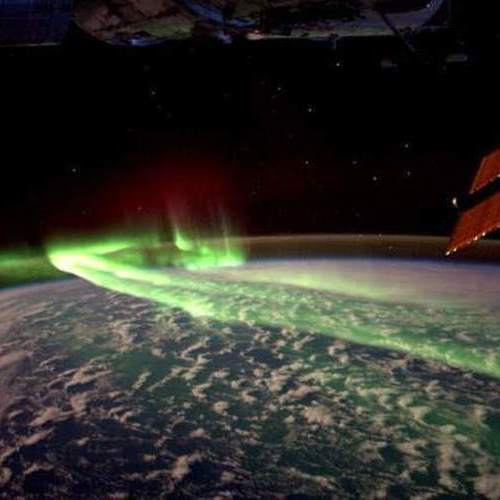
\includegraphics[width=100px]{/jungle/image03.jpg} \ \ \
			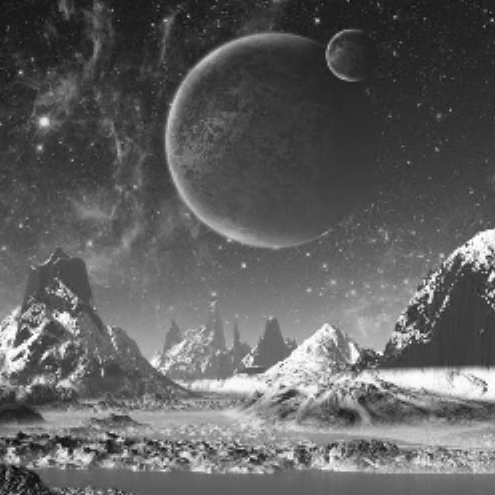
\includegraphics[width=100px]{/jungle/decompressed_13.png} \\
			\caption{À direita a imagem original e à esquerda a imagem após o processo. O erro obtido foi de 1.33\%.}  
		\end{figure}\par
		\begin{figure}[H]
			\centering
			\captionsetup{justification=centering}
			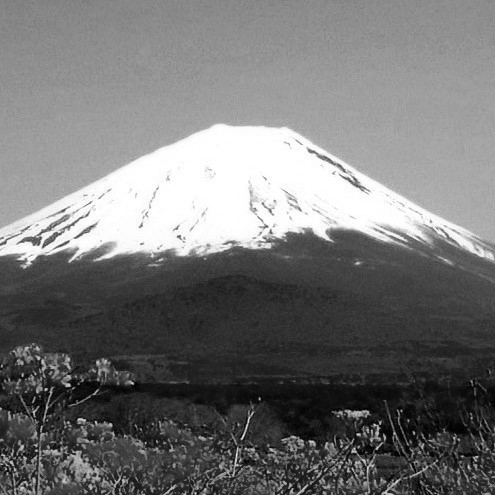
\includegraphics[width=100px]{/jungle/image04.jpg} \ \ \
			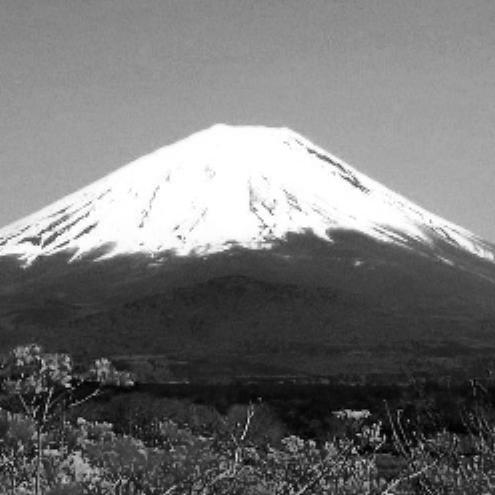
\includegraphics[width=100px]{/jungle/decompressed_14.png} \\
			\caption{À direita a imagem original e à esquerda a imagem após o processo. O erro obtido foi de 1.12\%.}  
		\end{figure}\par
		O erro obtido aqui foi pequeno para todas as imagens, porém, percebemos que o erro aumenta para as imagens preto e branco (funciona relativamente melhor para imagens coloridas) e além disso, possui um aumento quando a imagem tem muitas curvas (veja a figura 9).\par
		Comprimindo a imagem com $h$ maiores, obtemos imagens cada vez menores e, consequentemente, aumentamos o erro, bem como acontecia no Zoológico. Para constatar esse fato, comprimimos a imagem 1 com $k = 7$ e verificamos que o erro obtido foi de 5 \%. Esse valor de erro também foi observado quando comprimimos a imagem 1 três vezes com $k = 1$ e descomprimmimos três vezes com $k = 1$. Abaixo temos os resultados.
		\begin{figure}[H]
			\centering
			\captionsetup{justification=centering}
			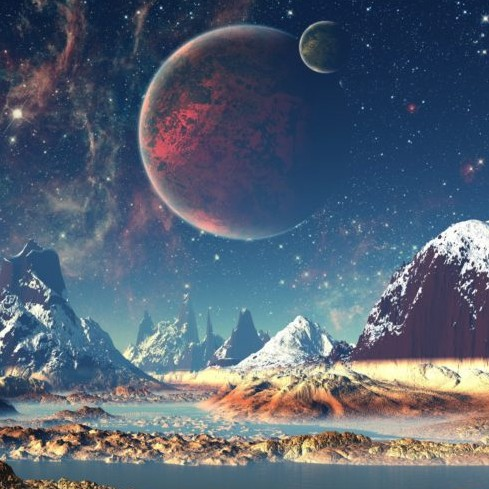
\includegraphics[width=100px]{/jungle/image01-k7.jpg} \ \ \
			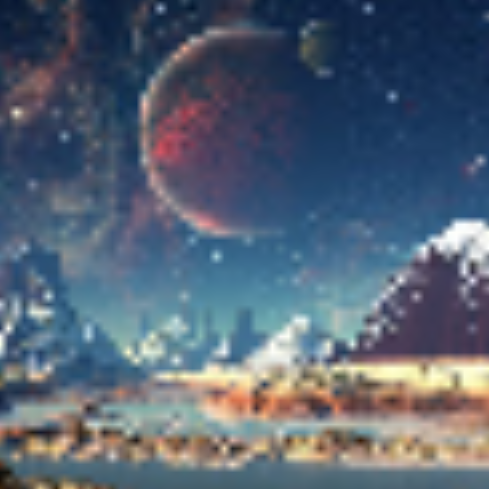
\includegraphics[width=100px]{/jungle/decompressed_1-k7-h1.png} \ \ \
			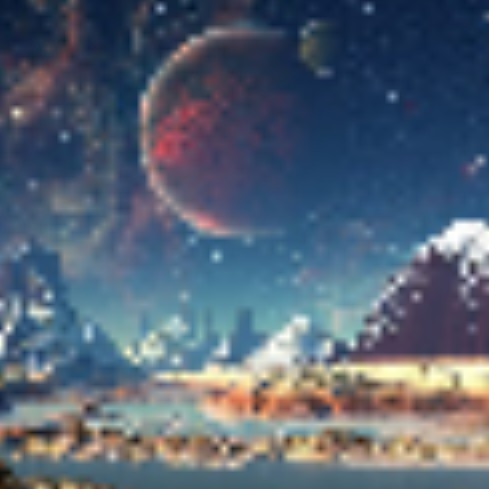
\includegraphics[width=100px]{/jungle/decompressed_1-k1-3-h1.png} \\
			\caption{À direita a imagem original, ao centro a imagem após uma compressão e descompressão com $k = 7$ e à esquerda a imagem após três compressões e três descompressões com $k = 1$.}  
		\end{figure}\par
	\pagebreak
	\section{Interpolação Bicúbica por partes}
	A ideia desse método é um pouco mais sofisticado que o anterior, pois aqui exigimos que a função seja suave e que a função interpoladora também o seja em todo o domínio da interpolação. \par
	Para entender o funcionamento, vamos considerar novamente os quatro pixels adjacentes $Q_{0}, Q_{1}, Q_{2}, Q_{3}$ com as mesmas coordenadas vistas anteriormente. Para interpolar um pixel que possui coordenadas $(x_{0}, y_{0})$ tal que $x_{0} \in [x_{i}, x_{i+1}]$ e $y_{0} \in [y_{j}, y_{j+1}]$, vamos interpolar a função $f$ geradora da imagem por uma função $v$ que interpolará também as primeiras derivadas em relação a x e y e a segunda derivada mista. Isso garante uma aproximação das derivadas (a suavidade da função deverá ser interpolada também). \par
	Em nossa implementação, porém, não tinhamos acesso as derivadas da função geradora da imagem $f$, por isso, para obte-la, usamos fórmulas que permitem aproximar esses valores. Nas bordas da imagem, utilizamos uma aproximação que leva em conta apenas um pixel a frente, a taxa de erro sendo $\mathcal{O}(h)$. No meio da imagem, usamos a fórmula centrada, que permite um erro de $\mathcal{O}(h^2)$, ou seja, uma aproximação melhor que nas bordas, entretanto, ficamos limitados com o erro das bordas. Vale lembrar que quanto menor for $h$, melhor será nossa aproximação e, consequentemente, nossa interpolação. Devemos apenas ficar atentos para escolha de um $h$ que seja suficientemente pequeno e que continue mantendo o erro de aproximação do método dominando o erro de arredondamento. Para manusear esses casos diferentes ao calcular as derivadas, implementamos uma \'moldura\' na matriz, repetindo a primeira e última linhas e colunas. Depois disso, varremos todos os pixels conhecidos, que são os índices da matriz (sem varrer os índices da moldura) e manuseamos a conta normalmente, pois ao referenciarmos índices que estariam fora da matriz, vamos acabar referenciando índices da moldura, que por serem os mesmos da primeira e última linhas e colunas, faz com que automaticamente estejamos utilizando o método de diferença lateral. Depois de calcularmos uma série de derivadas parciais e mistas, calculamos os coeficientes do polinômio e, usando uma estratégia similar a do caso bilinear (porém sem necessidade de modificar a fórmula, pois ela já permite isso), adicionamos mais linhas ao vetor X e mais colunas ao vetor Y para podermos calcular todos os pontos dentro do quadrado de uma vez só. Com isso, posicionamos o quadrado na matriz que se tornará a imagem interpolada, de modo idêntico ao bilinear.\par
	De forma semelhante ao visto no bilinear, como nosso algoritmo passa por cada um dos pixels, então podemos dizer que o tempo consumido é $\mathcal{O}(p^2)$, onde $p$ é a quantidade de pixels em na horizontal (ou vertical) da imagem original.
	
		\subsection{Resultados no Zoológico}
		Nossos experimentos no zoológico foram parecidos com os experimentos da interpolação bilinear por partes. Utilizamos as mesmas seis funções indicadas lá, porém, modificamos o valor de $h$, já que aqui quanto menor $h$ melhor será nossa interpolação (pois a aproximação da derivada será melhor). \par
		Fizemos os testes para $k = 1$ e $k = 5$, e verificamos que a alteração do valor de $h$ só tem impacto significativo para alguns testes com $k = 1$ (erro diminuiu aproximadamente $0.0001$\%). \par
		Abaixo, temos as imagens dos resultados das 6 funções com $h = 10^-4$ com os seus respectivos erros:
		
		\begin{figure}[H]
			\centering
			\captionsetup{justification=centering}
			
\includegraphics[width=100px]{/zoo/1.jpg} \ \ \
			
\includegraphics[width=100px]{/zoo/decompressed_21-h10^-4.png} \ \ \
			
\includegraphics[width=100px]{/zoo/decompressed_21-k5-h10^-4.png} \\
			\caption{Aqui temos a imagem original gerada pela função 1, a imagem após o processo com $k = 1$ (erro de 5.6\%) e a imagem após o processo com $k = 5$ (erro de 7.33\%).}  
		\end{figure}\par
		
		\begin{figure}[H]
			\centering
			\captionsetup{justification=centering}
			
\includegraphics[width=100px]{/zoo/2.jpg} \ \ \
			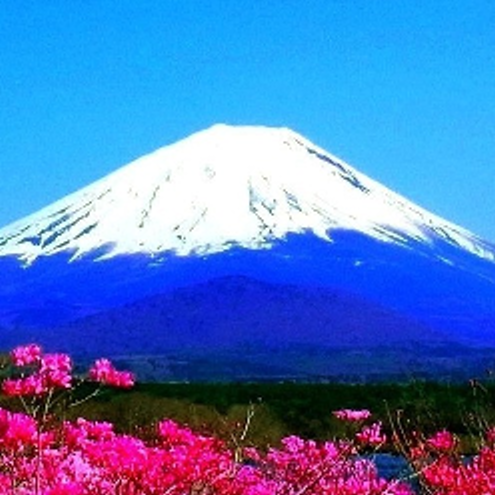
\includegraphics[width=100px]{/zoo/decompressed_22-k1-h10^-4.png} \ \ \
			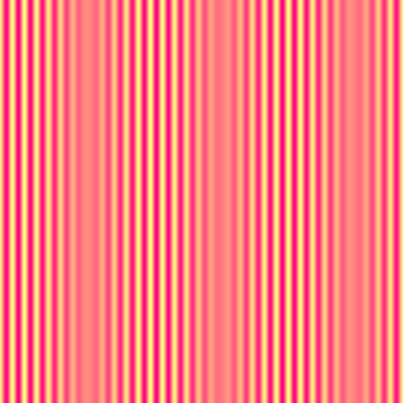
\includegraphics[width=100px]{/zoo/decompressed_22-k5-h10^-4.png} \\
			\caption{A imagem original gerada pela função 2, a imagem após o processo com $k = 1$ (erro de 5.3\%) e a imagem após o processo com $k = 5$ (erro de 12.5\%).}  
		\end{figure}\par
		
		\begin{figure}[H]
			\centering
			\captionsetup{justification=centering}
			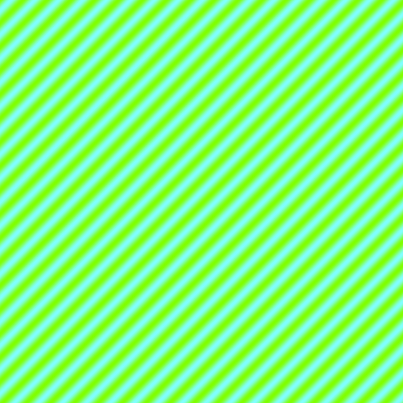
\includegraphics[width=100px]{/zoo/3.jpg} \ \ \
			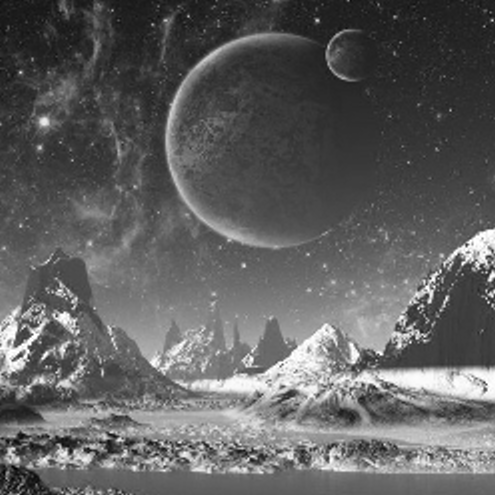
\includegraphics[width=100px]{/zoo/decompressed_23-k1-h10^-4.png} \ \ \
			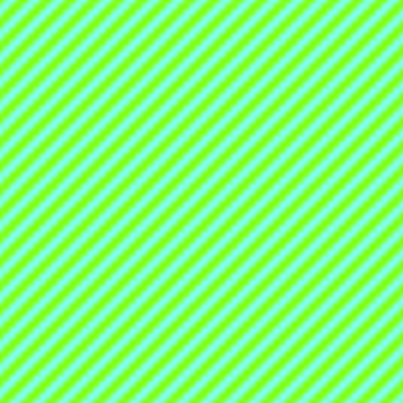
\includegraphics[width=100px]{/zoo/decompressed_23-k5-h10^-4.png} \\
			\caption{A imagem original gerada pela função 3, a imagem após o processo com $k = 1$ (erro de 0.1\%) e a imagem após o processo com $k = 5$ (erro de 2.6\%).}  
		\end{figure}\par
		Para a função 3, alterando $h$ obtivemos um erro menor (0.12020\% para $h = 1$, 0.12018\% para $h = 10^-4$, 0.12016\% para $h = 10^-6$).
		
		\begin{figure}[H]
			\centering
			\captionsetup{justification=centering}
			
\includegraphics[width=100px]{/zoo/4.jpg} \ \ \
			
\includegraphics[width=100px]{/zoo/decompressed_24-k1-h10^-4.png} \ \ \
			
\includegraphics[width=100px]{/zoo/decompressed_24-k5-h10^-4.png} \\
			\caption{A imagem original gerada pela função 4, a imagem após o processo com $k = 1$ (erro de 0.8\%) e a imagem após o processo com $k = 5$ (erro de 2.1\%).} 
		\end{figure}\par
		
		\begin{figure}[H]
			\centering
			\captionsetup{justification=centering}
			
\includegraphics[width=100px]{/zoo/5.jpg} \ \ \
			
\includegraphics[width=100px]{/zoo/decompressed_25-k1-h10^-4.png} \ \ \
			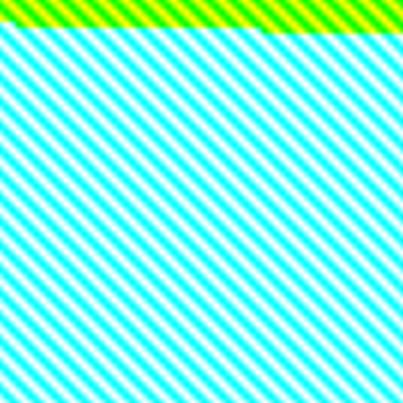
\includegraphics[width=100px]{/zoo/decompressed_25-k5-h10^-4.png} \\
			\caption{A imagem original gerada pela função 5, a imagem após o processo com $k = 1$ (erro de 0.6\%) e a imagem após o processo com $k = 5$ (erro de 3.8\%).} 
		\end{figure}\par
		\begin{figure}[H]
			\centering
			\captionsetup{justification=centering}
			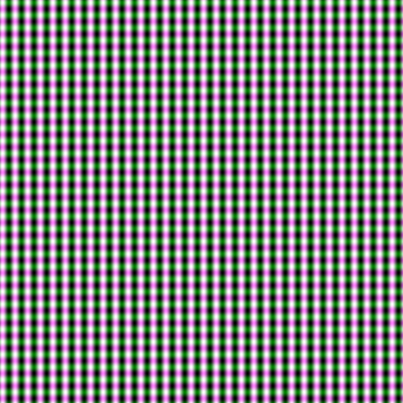
\includegraphics[width=100px]{/zoo/6.jpg} \ \ \
			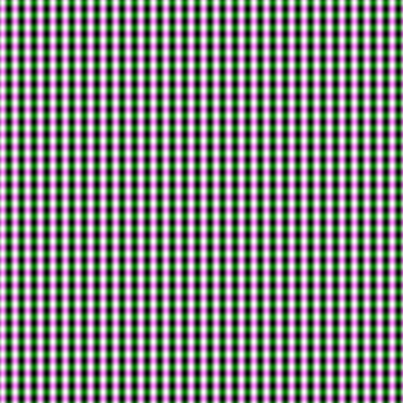
\includegraphics[width=100px]{/zoo/decompressed_26-k1-h10^-4.png} \ \ \
			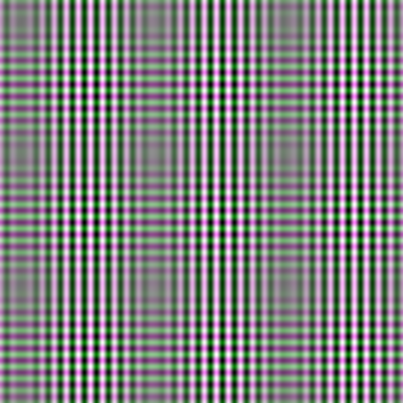
\includegraphics[width=100px]{/zoo/decompressed_26-k5-h10^-4.png} \\
			\caption{A imagem original gerada pela função 6, a imagem após o processo com $k = 1$ (erro de 0.8\%) e a imagem após o processo com $k = 5$ (erro de 3.1\%).} 
		\end{figure}\par
		É fácil perceber que as funções de classe $C^2$ tiveram um resultado bem melhor que as funções que não são. Isso se dá pelo fato de que essa interpolação considera as derivadas, garantindo, então, uma melhor aproximação para aquelas funções que são suaves e aumentando o erro daquelas que não são. Também vale notar que o erro aumenta ao passo que aumentamos o valor da compressão. \par
		Experimentamos, também, comprimir e descomprimir a imagem com $k = 7$ (obtemos erro de 54\%) e comprimir a imagem três vezes (erro de 55\%). O método bilinear obtém um erro menor do que esse para esses dois experimentos. \par
		Também percebemos que o erro não é alterado conforme diminuimos $h$ pela quantidade de informação que perdemos ao longo da compressão.\par
		Abaixo temos as imagens obtidas.

		\begin{figure}[H]
			\centering
			\captionsetup{justification=centering}
			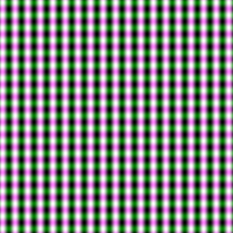
\includegraphics[width=100px]{/zoo/k7.jpg} \ \ \
			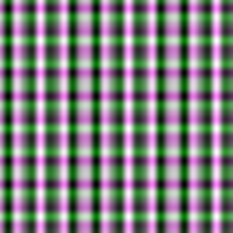
\includegraphics[width=100px]{/zoo/decompressed_2-k7-h10^-4.png} \ \ \
			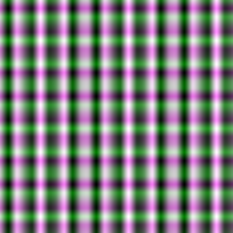
\includegraphics[width=100px]{/zoo/decompressed_2-k1-3-h10^-4.png} \\
			\caption{A imagem original gerada pela função 6, a imagem após o processo com $k = 7$ e a imagem após o processo de compressão três vezes e descompressão três vezes.} 
		\end{figure}\par
		
		\subsection{Resultados na Selva}
		Utilizamos, para os experimentos, as mesmas imagens utilizadas para o método bilinear. Da mesma forma que no zoológico, aqui não obtivemos diferenças quando variamos o valor de $h$. Para os testes, utilizamos apenas $k = 1$ e $h = 0.0001$. Os resultados seguem abaixo.
		\begin{figure}[H]
			\centering
			\captionsetup{justification=centering}
			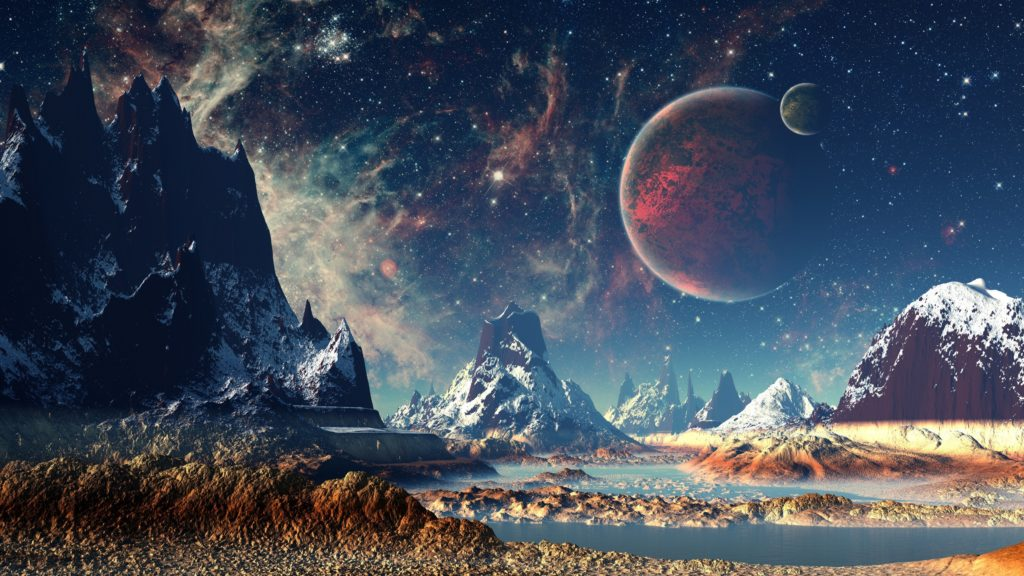
\includegraphics[width=100px]{/jungle/image01.jpg} \ \ \
			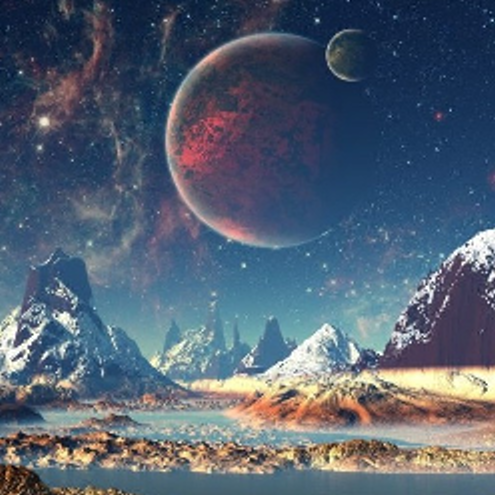
\includegraphics[width=100px]{/jungle/decompressed_21-k1-h10^-4.png} \\
			\caption{À direita a imagem original e à esquerda a imagem após o processo. O erro obtido foi de 1.3\%.}  
		\end{figure}\par
		\begin{figure}[H]
			\centering
			\captionsetup{justification=centering}
			\includegraphics[width=100px]{/jungle/image02.jpg} \ \ \
			\includegraphics[width=100px]{/jungle/decompressed_22-k1-h10^-4.png} \\
			\caption{À direita a imagem original e à esquerda a imagem após o processo. O erro obtido foi de 1\%.}  
		\end{figure}\par
		\begin{figure}[H]
			\centering
			\captionsetup{justification=centering}
			\includegraphics[width=100px]{/jungle/image03.jpg} \ \ \
			\includegraphics[width=100px]{/jungle/decompressed_23-k1-h10^-4.png} \\
			\caption{À direita a imagem original e à esquerda a imagem após o processo. O erro obtido foi de 1.3\%.}  
		\end{figure}\par
		\begin{figure}[H]
			\centering
			\captionsetup{justification=centering}
			\includegraphics[width=100px]{/jungle/image04.jpg} \ \ \
			\includegraphics[width=100px]{/jungle/decompressed_24-k1-h10^-4.png} \\
			\caption{À direita a imagem original e à esquerda a imagem após o processo. O erro obtido foi de 1\%.}  
		\end{figure}\par
		A qualidade da imagem é muito parecida com a do método bilinear, garantindo um erro pequeno tanto para imagens preto e branco quanto para imagens coloridas (com erro igual para os dois).\par
		Conforme feito no Zoológico, executamos o programa com $k = 7$ e também com $k = 1$ três vezes. Os resultados mostram um erro semelhante aos do caso bilinear (5\%). Abaixo temos as imagens obtidas.
		
		\begin{figure}[H]
			\centering
			\captionsetup{justification=centering}
			\includegraphics[width=100px]{/jungle/image01-k7.jpg} \ \ \
			\includegraphics[width=100px]{/jungle/decompressed_2-k7-h1.png} \ \ \
			\includegraphics[width=100px]{/jungle/decompressed_2-k1-3-h1.png} \\
			\caption{À direita a imagem original, ao centro a imagem após uma compressão e descompressão com $k = 7$ e à esquerda a imagem após três compressões e três descompressões com $k = 1$.}  
		\end{figure}\par
	
	\pagebreak
	\section{Conclusão}
	Com os testes tanto da selva quanto do zoológico, podemos concluir que as duas interpolações são suficientes para imagens com certas características, ou seja, quando precisamos ampliar uma imagem que tenha características mais curvas (aqui podemos dizer que a função geradora dessa imagem seria algo próximo de uma função de classe $C^2$), é mais interessante escolher o método bicúbico, já que os resultados obtidos para essa classe de funções foi bem melhor (um exemplo é a função 6 do zoológico, que nos mostrou um erro de aproximadamente 4\% para o método bilinear contra 0.8\% no bicúbico). Já para imagens que não tem características curvas, podemos utilizar o método bilinear, que é mais simples e relativamente mais rápido.
\end{document}